\documentclass[12pt,a4paper]{article}
\usepackage[utf8]{inputenc}
\usepackage[T1]{fontenc}
\usepackage[polish]{babel}
\usepackage{amsmath}
\usepackage{graphicx}
\usepackage{float}
\usepackage{geometry}
\geometry{margin=2.5cm}

\title{Sprawozdanie: Algorytmy Metaheurystyczne Lista 2}
\author{Wojciech Typer, nr indeksu 279730}
\date{\today}

\begin{document}

\maketitle

\section{Wstęp}
Poniższe sprawozdanie prezentuje wyniki implementacji i testów dwóch algorytmów metaheurystycznych: Symulowanego Wyżarzania (Simulated Annealing) oraz Przeszukiwania z Tabu (Tabu Search). 

Symulowane wyżarzanie to jedna z technik projektowania algorytmów heurystycznych. Cechą charakterystyczną tej metody jest występowanie parametru sterującego zwanego temperaturą, który maleje w trakcie wykonywania algorytmu. O sile eksploracji przestrzeni rozwiązań decyduje fakt, że z pewnym prawdopodobieństwem wyrażonym wzorem $e^{(f(X)-f(X^{\prime}))/T}$ może zostać zaakceptowane rozwiązanie gorsze.

Z kolei Tabu Search jest algorytmem, który rozszerza algorytm przeszukiwania lokalnego (Local Search) o mechanizm zabronień, czyli listę tabu. Mechanizm ten zapobiega wpadaniu w cykle i pozwala na opuszczenie ekstremum lokalnego.

\section{Zadanie 1: Symulowane Wyżarzanie}
\subsection{Dobór parametrów na małych danych}
Zgodnie z wymaganiami, algorytm symulowanego wyżarzania został poddany testom na małych i dużych zbiorach danych w celu ustalenia optymalnych parametrów startowych: początkowej wartości temperatury oraz współczynnika chłodzenia.

% tu daj wykres nr 1

\begin{figure}[H]
    \centering
    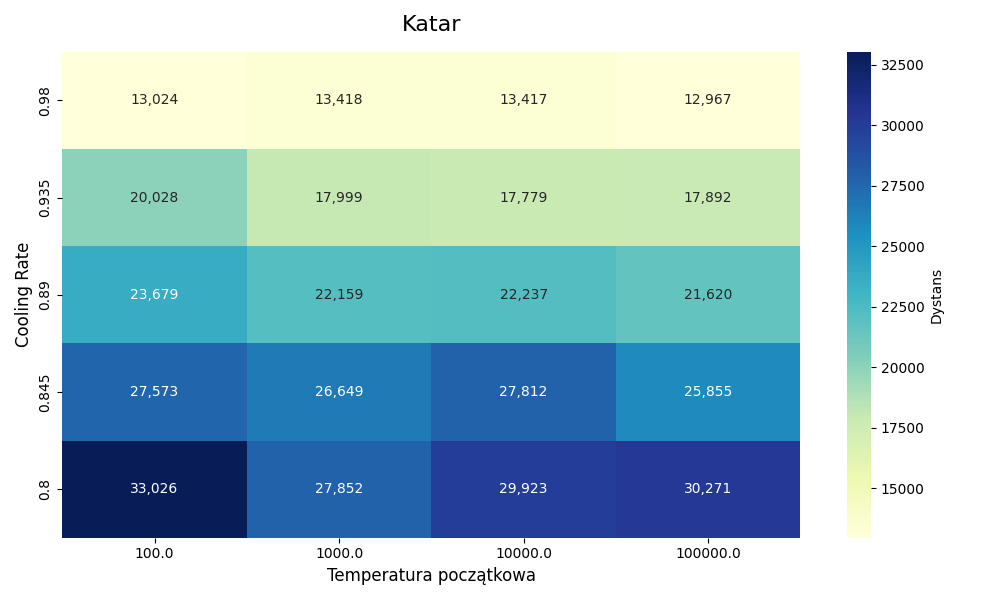
\includegraphics[width=0.8\textwidth]{../charts/Qatar1.png}
    \caption{Mapa cieplna wyników algorytmu Symulowanego Wyżarzania (dane Katar) w zależności od temperatury początkowej i współczynnika chłodzenia.}
    \label{fig:sa_params}
\end{figure}

\begin{figure}[H]
    \centering
    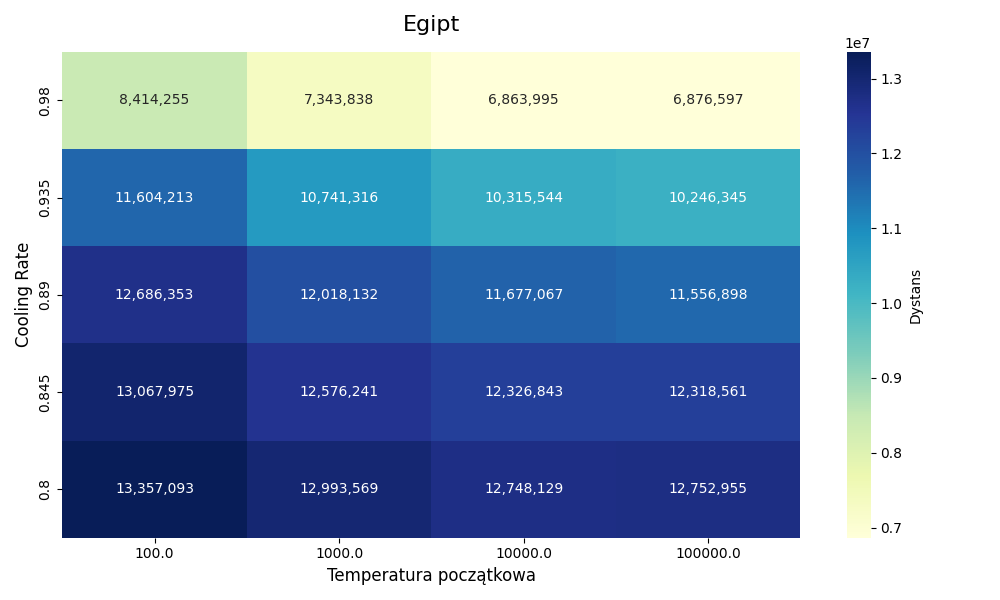
\includegraphics[width=0.8\textwidth]{../charts/Egipt1.png}
    \caption{Mapa cieplna wyników algorytmu Symulowanego Wyżarzania (dane Egypt) w zależności od temperatury początkowej i współczynnika chłodzenia.}
    \label{fig:sa_params}
\end{figure}

Dla wybranej dużej instancji problemu (Egipt) wykonano 100 prób obliczeniowych.
\begin{itemize}
    \item Najlepsze uzyskane rozwiązanie: 6863995
    \item Średnia wartość uzyskanych rozwiązań: 11 124 295.95
\end{itemize}

\begin{figure}[H]
    \centering
    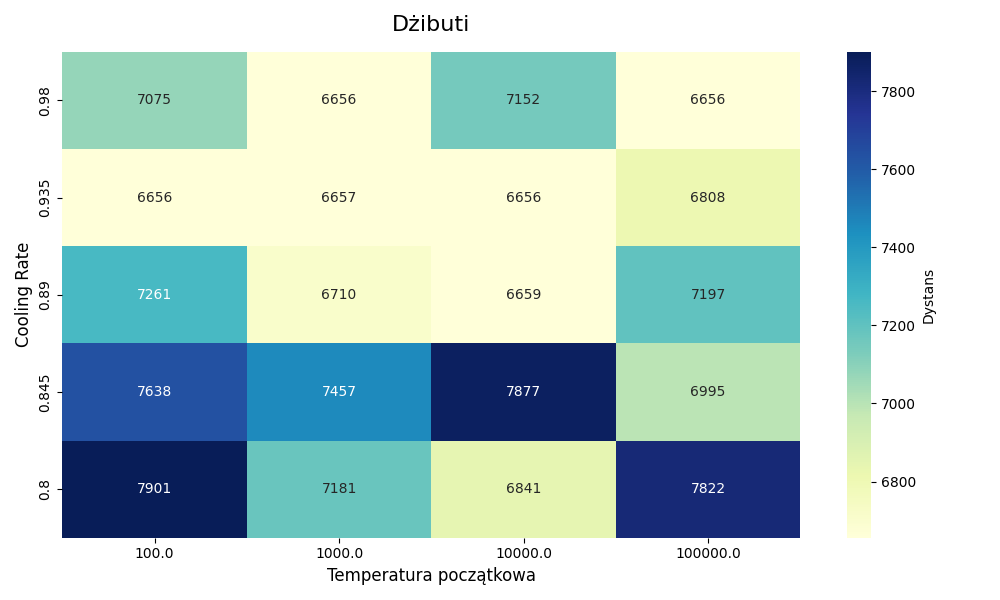
\includegraphics[width=0.8\textwidth]{../charts/Dzibuti1.png}
    \caption{Mapa cieplna wyników algorytmu Symulowanego Wyżarzania (dane Djibouti) w zależności od temperatury początkowej i współczynnika chłodzenia.}
    \label{fig:sa_params}
\end{figure}

Na podstawie przeprowadzonych eksperymentów i wygenerowanej mapy cieplnej można zauważyć, w których obszarach parametry radziły sobie najlepiej i osiągały minimum globalne (wartość 6656). Szybsze chłodzenie i stosunkowo wysoka temperatura początkowa pozwoliły na odpowiednią eksplorację bez marnowania czasu obliczeniowego.


\section{Zadanie 2: Tabu Search}
\subsection{Dobór parametrów na małych danych}
Drugim etapem była parametryzacja algorytmu Tabu Search dla małych danych. Testowanym parametrom podlegała długość listy tabu (tabu tenure) oraz warunek stopu wyrażony w maksymalnej liczbie iteracji bez poprawy (max stagnation).

% tu daj wykres nr 2
\begin{figure}[H]
    \centering
    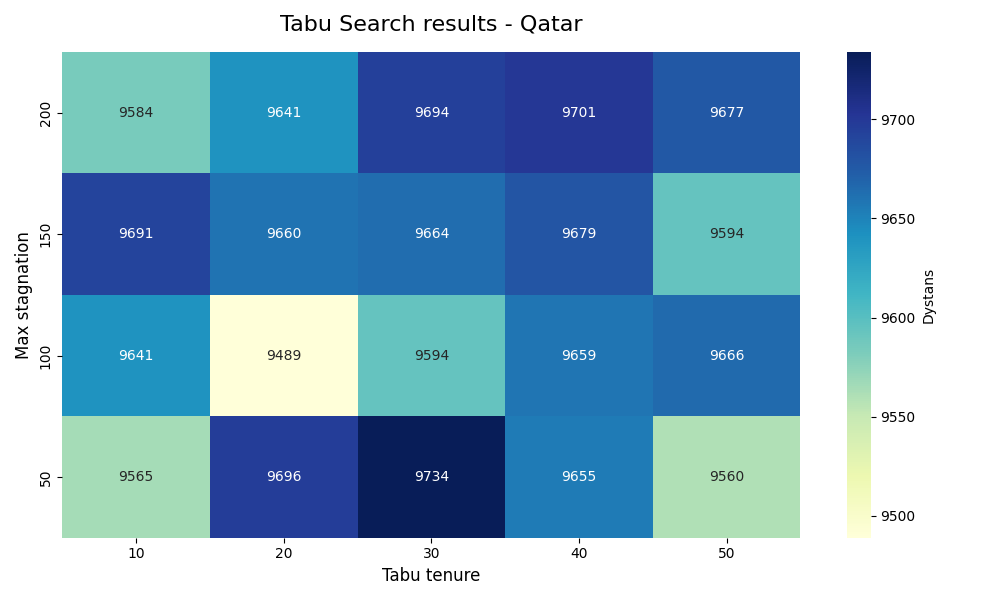
\includegraphics[width=0.8\textwidth]{../charts/Qatar2.png}
    \caption{Wpływ parametrów \textit{tabu tenure} i \textit{max stagnation} na ostateczny dystans w wariancie o zmiennych wynikach.}
    \label{fig:ts_params_var}
\end{figure}

Jak widać na powyższej wizualizacji, optymalną konfiguracją, która zwróciła wynik 9489, było ustawienie listy tabu na 20 przy zatrzymaniu stagnacji na 100 iteracjach. Następnie napotkano zjawisko widoczne na poniższym wykresie, gdzie parametry przestają mieć wpływ na wynik, co świadczy o szybkiej i silnej zbieżności do głębokiego ekstremum lokalnego.

% tu daj wykres nr 3
\begin{figure}[H]
    \centering
    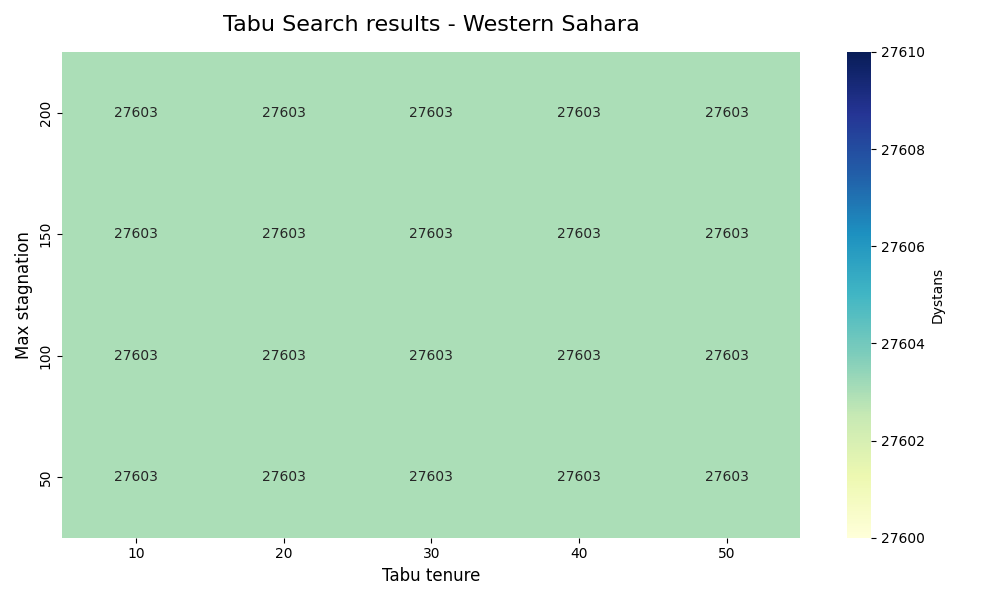
\includegraphics[width=0.8\textwidth]{../charts/WesternSahara.png}
    \label{fig:ts_params_uni}
\end{figure}

Identyczne wyniki dla wszystkich testowanych konfiguracji parametrów w algorytmie Tabu Search dla małych instancji problemu (np. Western Sahara) wynikają z następujących czynników:

\begin{enumerate}
    \item \textbf{Bardzo mała przestrzeń rozwiązań i prosty krajobraz (fitness landscape):} Przy niewielkiej liczbie miast liczba możliwych kombinacji dróg (oraz lokalnych minimów) jest na tyle mała, że algorytm bez problemu odnajduje najlepszą z nich. Powtarzający się wynik to najprawdopodobniej po prostu minimum globalne (optymalna trasa).
    
    \item \textbf{Deterministyczny i pełny przegląd sąsiedztwa:} Algorytm w każdym kroku sprawdza wszystkie możliwe pary sąsiadów (złożoność $\mathcal{O}(n^2)$) i wybiera najlepszą z nich. W małej przestrzeni powoduje to błyskawiczne i niemal natychmiastowe ,,zsunięcie się'' algorytmu na samo dno najlepszego lokalnego dołka, niezależnie od tego, z jakiej losowej trasy wystartował.
    
    \item \textbf{Marginalny wpływ parametrów:} Skoro algorytm znajduje optymalne rozwiązanie już w pierwszych iteracjach, to zwiększanie limitu stagnacji (\texttt{max\_stagnation}) z 50 na 200 nie zmienia wyniku -- algorytm po prostu dłużej wykonuje puste przebiegi wokół znalezionego już optimum, czekając na spełnienie warunku stopu. Podobnie rozmiar listy tabu (\texttt{tabu\_tenure}) jest na tyle duży w stosunku do liczby miast, że z łatwością zapobiega zapętleniom, gwarantując szybką zbieżność.
\end{enumerate}

\textbf{Podsumowując:} Dla bardzo małych zbiorów danych algorytm Tabu Search z pełnym przeglądem sąsiedztwa jest na tyle silny, że działa deterministycznie i błyskawicznie znajduje optymalną trasę. Z tego powodu manipulacja badanymi parametrami nie przynosi żadnych widocznych różnic w ostatecznym dystansie.

\section{Porównanie skuteczności i czasu działania metod}
Ostatnim punktem analizy było porównanie skuteczności oraz czasów działania aktualnych metod z tymi zaimplementowanymi na poprzedniej liście.

Algorytm Tabu Search jest dokładniejszy, ale sporo wolniejszy od algorytmu Symulowanego Wyżarzania. Wyższa dokładność oznacza, że najlepsze znalezione rozwiązanie w przypadku Tabu Search charakteryzuje się lepszą jakością (krótszym dystansem) niż w przypadku Wyżarzania. 

Z kolei algorytm lokalnego przeszukiwania (Local Search) z pierwszej listy jest sporo dokładniejszy, a zarazem dużo wolniejszy od algorytmu Tabu Search.

\end{document}